% generated by scripts/pkl_to_latex.py
% source PKL : thermal_v1_L6_Ne6_U10_t1_mode-uniform_tpall_t2all_tperpall_nmin2_solver-gcg_restarts2_iter200_kmax4_tol1em09_cut10_adaptive1_step5_clusteravg1_T0.01to5_N40-51abceee4722_knone_diag0.pkl
% scan type  : Tscan
% state      : gs
% requires   : \usepackage{pgfplots} \pgfplotsset{compat=1.18}
% colours match the matplotlib PDF (tab10 cycle)
\definecolor{gmeC0}{HTML}{1F77B4}
\definecolor{gmeC1}{HTML}{FF7F0E}
\definecolor{gmeC2}{HTML}{2CA02C}
\definecolor{gmeC3}{HTML}{D62728}
\definecolor{gmeC4}{HTML}{9467BD}
\definecolor{gmeC5}{HTML}{8C564B}
\definecolor{gmeC6}{HTML}{E377C2}
\definecolor{gmeC7}{HTML}{17BECF}

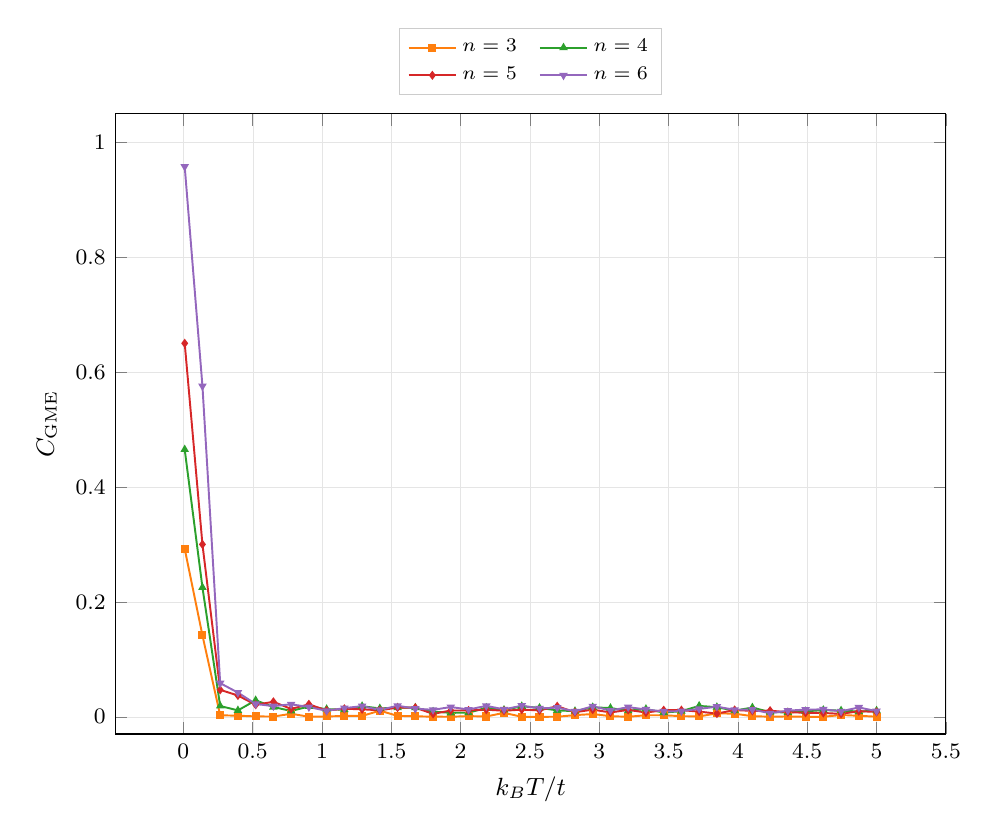
\begin{tikzpicture}
  \begin{axis}[
    width=\columnwidth,
    height=0.78\columnwidth,
    xlabel={$k_B T/t$},
    ylabel={$C_{\mathrm{GME}}$},
    grid=both,
    grid style={line width=.1pt, draw=gray!20},
    tick label style={font=\footnotesize\rmfamily, /pgf/number format/fixed},
    label style={font=\small\rmfamily},
    scaled ticks=false,
    legend style={font=\scriptsize\rmfamily, draw=gray!40, at={(0.5,1.03)}, anchor=south, /tikz/every even column/.append style={column sep=6pt}},
    legend cell align={left},
    legend columns=2,
    ymin=-0.03,
    ymax=1.05,
  ]
    \addplot[color=gmeC1, mark=square*, mark size=1.1pt, line width=0.7pt] coordinates {
        (0.01,0.292503) (0.137949,0.141765) (0.265897,0.002667) (0.393846,0.001905)
        (0.521795,0.000724) (0.649744,0.000457) (0.777692,0.005261) (0.905641,0.000135)
        (1.03359,0.000569) (1.161538,0.001567) (1.289487,0.001518) (1.417436,0.010703)
        (1.545385,0.001639) (1.673333,0.000863) (1.801282,0.000224) (1.929231,0.0001)
        (2.057179,0.001228) (2.185128,0.000543) (2.313077,0.006934) (2.441026,0.000007)
        (2.568974,0) (2.696923,0.000093) (2.824872,0.002948) (2.952821,0.004796)
        (3.080769,0.001131) (3.208718,0.000008) (3.336667,0.002756) (3.464615,0.0027)
        (3.592564,0.001081) (3.720513,0.000633) (3.848462,0.00606) (3.97641,0.005439)
        (4.104359,0.001077) (4.232308,0.000182) (4.360256,0.000604) (4.488205,0.000002)
        (4.616154,0.000049) (4.744103,0.003139) (4.872051,0.001801) (5,0.00018)
    };
    \addlegendentry{$n=3$}
    \addplot[color=gmeC2, mark=triangle*, mark size=1.1pt, line width=0.7pt] coordinates {
        (0.01,0.465518) (0.137949,0.225243) (0.265897,0.018829) (0.393846,0.011158)
        (0.521795,0.02871) (0.649744,0.017041) (0.777692,0.010179) (0.905641,0.017938)
        (1.03359,0.013234) (1.161538,0.012368) (1.289487,0.018423) (1.417436,0.014609)
        (1.545385,0.015884) (1.673333,0.01587) (1.801282,0.008933) (1.929231,0.006971)
        (2.057179,0.007127) (2.185128,0.015662) (2.313077,0.011889) (2.441026,0.018354)
        (2.568974,0.015559) (2.696923,0.011253) (2.824872,0.009804) (2.952821,0.016592)
        (3.080769,0.015189) (3.208718,0.010585) (3.336667,0.013458) (3.464615,0.007454)
        (3.592564,0.009789) (3.720513,0.018995) (3.848462,0.01671) (3.97641,0.010762)
        (4.104359,0.016128) (4.232308,0.008148) (4.360256,0.007693) (4.488205,0.009587)
        (4.616154,0.011703) (4.744103,0.010774) (4.872051,0.009175) (5,0.010638)
    };
    \addlegendentry{$n=4$}
    \addplot[color=gmeC3, mark=diamond*, mark size=1.1pt, line width=0.7pt] coordinates {
        (0.01,0.650363) (0.137949,0.300278) (0.265897,0.046972) (0.393846,0.037118)
        (0.521795,0.020909) (0.649744,0.026145) (0.777692,0.01373) (0.905641,0.021775)
        (1.03359,0.010981) (1.161538,0.013983) (1.289487,0.013106) (1.417436,0.011317)
        (1.545385,0.016105) (1.673333,0.015886) (1.801282,0.005167) (1.929231,0.010982)
        (2.057179,0.011082) (2.185128,0.012384) (2.313077,0.010613) (2.441026,0.012457)
        (2.568974,0.011247) (2.696923,0.018408) (2.824872,0.00797) (2.952821,0.012528)
        (3.080769,0.007571) (3.208718,0.012068) (3.336667,0.007487) (3.464615,0.011498)
        (3.592564,0.011585) (3.720513,0.009032) (3.848462,0.005631) (3.97641,0.011807)
        (4.104359,0.010285) (4.232308,0.010709) (4.360256,0.007983) (4.488205,0.007111)
        (4.616154,0.006692) (4.744103,0.005102) (4.872051,0.009795) (5,0.008544)
    };
    \addlegendentry{$n=5$}
    \addplot[color=gmeC4, mark=triangle*, mark size=1.1pt, mark options={rotate=180}, line width=0.7pt] coordinates {
        (0.01,0.958182) (0.137949,0.575954) (0.265897,0.058575) (0.393846,0.04219)
        (0.521795,0.022337) (0.649744,0.018636) (0.777692,0.021806) (0.905641,0.016968)
        (1.03359,0.010432) (1.161538,0.015185) (1.289487,0.018539) (1.417436,0.011987)
        (1.545385,0.019273) (1.673333,0.014201) (1.801282,0.012174) (1.929231,0.016999)
        (2.057179,0.012719) (2.185128,0.018993) (2.313077,0.013024) (2.441026,0.01931)
        (2.568974,0.014553) (2.696923,0.01603) (2.824872,0.009542) (2.952821,0.018323)
        (3.080769,0.010988) (3.208718,0.016805) (3.336667,0.012772) (3.464615,0.009347)
        (3.592564,0.009928) (3.720513,0.013782) (3.848462,0.017679) (3.97641,0.012168)
        (4.104359,0.0126) (4.232308,0.006188) (4.360256,0.010738) (4.488205,0.012526)
        (4.616154,0.01294) (4.744103,0.009643) (4.872051,0.016266) (5,0.009939)
    };
    \addlegendentry{$n=6$}
  \end{axis}
\end{tikzpicture}
